\documentclass{article}
\usepackage{pgfplots}
\title{KEEL: ROC output}
\begin{document}
\maketitle
\pagebreak[4]
\hfill \break
Section one: TEST FILE
\hfill \break
\hfill \break
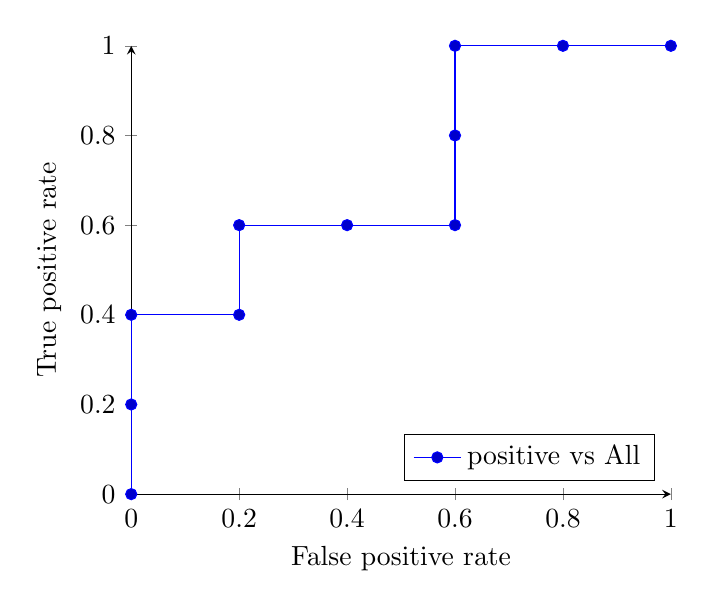
\begin{tikzpicture}
\begin{axis} [xlabel=False positive rate,
ylabel=True positive rate,axis x line=bottom,
axis y line=left, legend pos=south east]
\addplot coordinates { (0,0)(0.0,0.2)(0.0,0.4)(0.2,0.4)(0.2,0.6000000000000001)(0.4,0.6000000000000001)(0.6000000000000001,0.6000000000000001)(0.6000000000000001,0.8)(0.6000000000000001,1.0)(0.8,1.0)(1.0,1.0)};\addlegendentry{positive vs All}
\end{axis}
\end{tikzpicture}\hfill \break
\hfill \break
 Area Under Curve (AUC):0.72
\hfill \break
\hfill \break
\end{document}